% LLM-DoW-Bench -- SaTML 2027 submission
%
% Anonymized for double-blind review per SaTML 2027 CFP:
% no author names/institutions anywhere in this file.

\documentclass[conference]{IEEEtran}
\usepackage{cite}
\usepackage{graphicx}
\usepackage{amsmath,amssymb}
\usepackage{url}
\usepackage{booktabs}
\usepackage{pgfplots}
\pgfplotsset{compat=1.18}

\begin{document}

\title{LLM-DoW-Bench: A Benchmark and Threat Model for Denial-of-Wallet Attacks Against LLM Tool-Use Agents}

% Double-blind: no author block.
\author{\IEEEauthorblockN{Anonymous Author(s)}
\IEEEauthorblockA{Submitted to IEEE SaTML 2027}}

\maketitle

\begin{abstract}
LLM agents with tool access can be induced, via indirect prompt injection or adversarial task framing, into consuming far more cost than a task warrants -- without any individually unauthorized action. We term this a \emph{Denial-of-Wallet (DoW)} attack: the victim's systems remain available; only their bill is affected. Because every action is individually permitted, action-legitimacy defenses do not obviously transfer, and existing agent-security benchmarks measure only behavioral compromise, never cost. We present LLM-DoW-Bench: a taxonomy of six cost-amplification vectors spanning two agentic task domains, and a LangGraph-based cost-metering harness. We evaluate six frontier models across five trials per condition for five of the six vectors; the sixth (adversarial task framing, no injection) is included in the taxonomy but not yet validly instrumented, which we report as a negative methodological result. Cost-amplification is sharply heterogeneous: context/input bloat amplifies cost severely for every model (mean $6.4\times$, up to $21.5\times$), while retry induction and expensive-tool bait are weak (mean $1.2$--$1.3\times$). The two delegation vectors show a per-model split: four of six models resist injected delegation instructions almost perfectly, while two OpenAI models comply substantially. We evaluate two of four candidate defenses: a hard cumulative-cost budget and an intent-consistency LLM judge. Contrary to prediction, the budget is nearly inert (0.7\% attack-block rate): our pre-tool-call gate cannot intervene on cost accrued within a single call, the mechanism the dominant vector exploits. The intent judge, predicted to show less resistance, instead blocks more attack trials (13.3\%), but only for the delegation vectors and models already susceptible to them, at a small false-positive cost. Both defenses leave the dominant vector untouched.
\end{abstract}

\begin{IEEEkeywords}
LLM agents, prompt injection, denial of wallet, resource exhaustion, economic denial of sustainability, agent security benchmarks
\end{IEEEkeywords}

\section{Introduction}
\label{sec:intro}

LLM agents with tool access -- shell execution, cloud APIs, database queries, paid third-party APIs, sub-agent spawning -- are increasingly deployed to complete multi-step tasks with limited human supervision. This autonomy creates an attack surface distinct from the one usually discussed for prompt injection. The standard framing of indirect prompt injection concerns an agent tricked, via untrusted content it reads, into taking an unauthorized or harmful action: exfiltrating data, executing a destructive command, or violating an access boundary. That framing assumes the harm is legible as a rule violation -- some action the agent took was not permitted.

A different failure mode does not require any rule violation at all. An agent can be induced, by the same delivery mechanisms (a poisoned tool result, a page it is asked to summarize, an adversarially framed task), into doing something entirely permitted -- searching, calling an API, delegating to a sub-agent -- an excessive number of times, or in an unnecessarily expensive way. No confidentiality or integrity boundary is crossed. The agent's owner simply pays for work the task did not need. We refer to this as a Denial-of-Wallet (DoW) attack against LLM tool-use agents, adopting a term with an established academic lineage in serverless-computing security~\cite{kelly2021dow,dorsett2025dowreview,dorsett2025dowtaxonomy} and separately reapplied, informally, in generative-AI industry security writing~\cite{promptsecurity2025dow}. Two concurrent 2026 papers, Zhou et al.~\cite{zhou2026toolchain} and SkillBloat~\cite{skillbloat2026}, independently measure cost/token amplification through an agent-adjacent channel, but under threat models and with a scope this paper's contribution is specifically positioned against (Section~\ref{sec:related}). A recent systematization of knowledge on the agentic-AI attack surface, Dehghantanha et al.~\cite{dehghantanha2026sok}, surveys prompt-injection, knowledge-base-poisoning, tool/plugin-exploit, and multi-agent threats broadly and proposes its own evaluation metrics (Unsafe Action Rate, Privilege Escalation Distance), but does not address cost- or resource-exhaustion attacks, and its proposed metrics target unsafe or privileged actions rather than economic cost -- underscoring that even a broad, recent systematization of the agentic-AI threat landscape does not yet cover the failure mode this paper studies. To our knowledge, no existing work combines an indirect-prompt-injection-style threat model, a taxonomy spanning both single-agent and multi-agent/delegation vectors, and a reusable, cost-instrumented benchmark with a paired defense evaluation, for the agentic tool-use setting.

This failure mode has a non-adversarial counterpart: OWASP's LLM Top 10 explicitly names ``Unbounded Consumption'' as a production risk for LLM deployments, noting that unintentional retry loops, unmonitored tool invocations, and uncapped agent fan-out create the same cost exposure that our adversarial corpus targets~\cite{owasp2025llm10}. Our interest is the adversarial version of that same exposure: an attacker who deliberately engineers a task, document, or tool response to maximize an agent's cost.

\textbf{Why existing defenses don't obviously transfer.} Intent-consistency checks and permission-scoping mechanisms are built to catch an action that should not have been taken at all. A DoW attack does not require such an action -- every individual tool call can be exactly the kind of call the agent's permissions were designed to allow. This is the cost-specific instance of a more general point independently argued by Lotfi et al.~\cite{lotfi2026trajectory} for regulatory/behavioral-compliance invariants: a sequence of individually permitted agent actions can collectively violate a trajectory-level invariant that no single-action check can see. Section~\ref{sec:defenses} runs an actual defense evaluation against this prediction, and the result is more mixed than the clean hypothesis above: an intent-consistency judge does show some attack-resistance (not none), while a budget-aware hard cap shows almost no resistance at all, for a structural reason (Section~\ref{sec:defenses}) rather than because budgets are inherently weak.

\textbf{Why existing benchmarks don't measure this.} We reviewed four widely cited, methodologically rigorous agent-security benchmarks -- AgentDojo~\cite{debenedetti2024agentdojo}, InjecAgent~\cite{zhan2024injecagent}, ToolEmu~\cite{ruan2024toolemu}, and R-Judge~\cite{yuan2024rjudge} -- and confirmed that none of them instrument for token count, tool-call count, dollar cost, wall-clock time, or sub-agent fan-out as an evaluation outcome. Their outcome variable is uniformly behavioral compromise (an unauthorized or harmful action) or data exfiltration, not economic exhaustion. Two concurrent 2026 works do measure cost/token amplification directly -- Zhou et al.~\cite{zhou2026toolchain} via a malicious-MCP-server threat model on single-tool tasks, and SkillBloat~\cite{skillbloat2026} via malicious skill-file injection in coding agents -- but neither evaluates multi-agent delegation, and neither releases a reusable, multi-domain benchmark artifact of the kind this paper contributes (Section~\ref{sec:related}).

\textbf{Contributions.}
\begin{itemize}
\item A threat model for DoW attacks against LLM tool-use agents specifically, distinguishing this attack surface from (a) classical resource-exhaustion / Economic Denial of Sustainability (EDoS) attacks on non-agentic cloud infrastructure~\cite{baig2013edos}, (b) existing LLM-level denial-of-service attacks that target the base model or serving stack directly rather than the tool-use/orchestration layer~\cite{gao2024dospoisoning,liu2026reasoningbomb,wang2026latencydos,bilal2026nonhalting}, and (c) concurrent tool-layer cost-amplification work that assumes a stronger (server-compromise or single-product-feature) adversary and does not cover multi-agent delegation~\cite{zhou2026toolchain,skillbloat2026} (Section~\ref{sec:threatmodel}).
\item LLM-DoW-Bench: a reproducible benchmark comprising an attack corpus of six vectors across two agentic task domains and a LangGraph-based cost-metering harness (Section~\ref{sec:methodology}).
\item An empirical evaluation of six frontier tool-use agent configurations' susceptibility to DoW attacks across five trials per condition, measured by cost-amplification factor for five of the six taxonomy vectors (V1--V4, V6), finding sharp vector- and model-dependent heterogeneity rather than a uniform effect; the sixth vector's (V5) corpus entry is diagnosed as not yet validly instrumented, which we report as a methodological finding in its own right rather than omit (Section~\ref{sec:evaluation}).
\item A defense evaluation (Section~\ref{sec:defenses}) of two candidate defenses -- a hard cumulative-cost budget and an intent-consistency LLM-judge -- against this corpus, finding that neither provides the clean, uniform "meaningful resistance" our own threat model predicted for budget-aware mechanisms, and that a pre-tool-call gate architecture (the natural implementation for both defense classes) is structurally unable to intervene on the specific vector (V4, context/input bloat) that causes the most severe cost amplification in Section~\ref{sec:evaluation}.
\end{itemize}

\section{Related Work}
\label{sec:related}

\subsection{Indirect Prompt Injection and Agent-Security Benchmarks}

Indirect prompt injection -- an agent's behavior redirected by adversarial content embedded in data it processes, rather than by an instruction from its principal -- is well established as an attack class. AgentDojo~\cite{debenedetti2024agentdojo} evaluates 97 realistic agent tasks against 629 security test cases across email, banking, and travel-booking-style environments; InjecAgent~\cite{zhan2024injecagent} evaluates 1,054 test cases across 30 agents, categorizing outcomes into direct user harm and private data exfiltration; ToolEmu~\cite{ruan2024toolemu} uses an LM-emulated sandbox across 36 tools and 144 scenarios to surface safety failures; R-Judge~\cite{yuan2024rjudge} evaluates whether models can recognize safety risk in 569 multi-turn agent interaction records across 10 risk types. The largest and most recent benchmark in this space, Agent Security Bench (ASB)~\cite{zhang2025asb}, spans 10 scenarios, 10 agents, over 400 tools, and 27 attack/defense types across 7 evaluation metrics. We verified, by reviewing each benchmark's methodology directly, that none of these five measures token count, tool-call count, dollar cost, or fan-out depth as an outcome variable -- ASB's metrics center on attack success rate (up to 84.3\%) and a utility-security balance score, not economic exhaustion. All five treat the outcome of an attack as a behavioral or data-integrity compromise, not an economic one. A sixth, concurrent 2026 benchmark, AgentLAB~\cite{jiang2026agentlab}, evaluates 644 test cases across 28 environments against five long-horizon attack categories, one of which -- tool chaining -- mechanistically overlaps with this paper's delegation vectors (V2, V6); however, AgentLAB's outcome metric is attack success rate, not cost or token amplification, so it does not close the gap this paper targets. This project targets that specific gap: an equally rigorous benchmark whose outcome variable is cost.

\subsection{Cost-Amplification Attacks Through the Tool-Use Layer (Concurrent Work)}
\label{sec:concurrent}

Two concurrent 2026 papers attack cost through the tool-calling layer specifically, the same layer this paper targets, and are the closest existing work to our contribution. Zhou et al.~\cite{zhou2026toolchain} assume an adversary who controls a malicious MCP tool \emph{server} and rewrites its response templates -- a supply-chain-adjacent capability, not an indirect-prompt-injection one -- and use Monte Carlo Tree Search to synthesize multi-turn tool-calling chains that inflate cost by up to 658$\times$ on single-tool, single-turn subsets of ToolBench and BFCL; they evaluate several defenses (perplexity filters, self-reflection monitoring, trajectory-level safety judges, hard budget caps), all evaded or only partially effective, but release an attack-generation method rather than a reusable benchmark artifact, and do not address multi-agent delegation. SkillBloat~\cite{skillbloat2026} targets a narrower channel -- the "Agent Skills" feature of coding agents specifically -- using an automated two-phase framework to rewrite a skill document for maximum token amplification, reporting 5.4$\times$--10.1$\times$ average best amplification; it likewise does not address multi-agent delegation or evaluate defenses. Both works confirm that cost/token amplification through an agent-adjacent channel is measurable and severe, which motivates rather than undercuts this paper's contribution. A third concurrent work, LeechHijack~\cite{leechhijack2025}, hijacks agent compute for attacker-specified tasks via a backdoored Model Context Protocol (MCP) tool exhibiting "implicit toxicity" -- exploiting granted permissions without privilege escalation -- reporting an 18.6\% token-cost overhead and 77.3\% average attack success across model families; like Zhou et al., it assumes a compromised tool rather than merely poisoned content an otherwise-trustworthy tool returns, and releases no reusable benchmark artifact. For the multi-agent setting specifically, CORBA~\cite{corba2025} is the closest identified prior work to our delegation-loop vector (V6): a "contagious" attack that propagates across arbitrary multi-agent network topologies via ordinary message-passing (no delegation-tool primitive required) and a "recursive" self-loop property that sustains computational-resource depletion via seemingly benign instructions. We read CORBA in full and confirm it measures a fundamentally different asset than ours: its outcome metrics are Proportional Attack Success Rate (the fraction of agents driven to stop responding, up to 100\%) and Peak Blocking Turn Number -- an availability/blocking metric, not an economic one -- and it reports no cost, token, or dollar-amplification ratio. V6 measures whether a functioning agent's \emph{cost} is amplified by unbounded delegation depth; CORBA measures whether agents stop responding at all. We treat this as complementary rather than competing: CORBA and this paper study different STRIDE-adjacent harms (availability vs. budget) arising from structurally similar multi-agent propagation dynamics.

Our threat model differs from all four in three respects: (1) we assume only the standard indirect-prompt-injection capability already used by AgentDojo, InjecAgent, and ToolEmu (C1: poisoned content the agent reads via an otherwise-legitimate tool call) or an adversarially framed task (C2), not server/tool compromise or a single vendor-specific feature; (2) our taxonomy explicitly includes sub-agent fan-out (V2) and delegation-loop induction (V6) under this weaker capability assumption, whereas CORBA's multi-agent attack requires no injection channel comparison to be drawn until its full text is read; and (3) we contribute a reusable, cost-instrumented benchmark spanning two task domains with a paired defense evaluation, rather than an attack-generation method evaluated on synthetic single-tool stubs or a proof-of-concept backdoor. This concentration of concurrent 2025--2026 work is consistent with a broader diagnosis from a recent survey on resource-consumption threats in LLMs~\cite{zhang2026resourcesurvey}, which characterizes this as an emerging area still lacking a unified problem framing and calls for a clearer foundation for characterizing and mitigating such threats across the full pipeline from threat induction to mitigation -- a gap this paper's cost-instrumented, multi-agent-delegation-aware benchmark and paired defense evaluation is a step toward closing.

\subsection{LLM-Level and Infrastructure-Level Denial-of-Service}

A separate line of work has shown LLMs and their serving infrastructure vulnerable to denial-of-service and cost-inflation attacks that operate below the tool-use/orchestration layer. Gao et al.~\cite{gao2024dospoisoning} poison fine-tuning data with a single sample to force excessively long generations (up to 16{,}384 tokens) on trigger, demonstrated on GPT-4o for under \$1, and explicitly discuss an LLM-agent deployment scenario as one of three threat settings. Liu et al.~\cite{liu2026reasoningbomb} (ReasoningBomb) formalize prompt-induced inference-time denial-of-service against reasoning models, using reinforcement learning to craft short prompts that induce pathologically long reasoning traces, and explicitly frame the resulting cost asymmetry between flat subscription pricing and variable inference cost. Wang et al.~\cite{wang2026latencydos} attack the LLM serving framework itself (scheduler state, KV cache) rather than the model, achieving substantial time-to-first-token slowdowns. Hammouri et al.~\cite{bilal2026nonhalting} (Non-Halting Queries, SaTML 2025) exploit fixed points in autoregressive models: if the output repeats a cyclic token sequence beyond the context window it never reaches the end-of-string token, and they demonstrate prompts that induce this state in every major aligned model with success rates as high as 97\%. Kumar et al.~\cite{kumar2025overthink} (OverThink) mount slowdown attacks on reasoning LLMs by injecting benign-appearing decoy reasoning problems (Markov decision processes, Sudokus) into context the model consumes, substantially inflating reasoning-token overhead without degrading answer quality or triggering safety filters. Dong et al.~\cite{engorgio2024} (Engorgio, ICLR 2025) suppress the end-of-string token directly via a parameterized distribution objective, inducing 2--13$\times$ longer outputs across 13 open-source models in a white-box setting. Zhou, Wang, Ma, et al.~\cite{shieldtotarget2026} attack an LLM-based agent \emph{guardrail} rather than the primary agent, trapping it in extended reasoning loops via a single poisoned document to achieve 13--63$\times$ token and up to 148$\times$ latency amplification -- notably using the same delivery mechanism as our C1, but against a safety-filter component rather than the task-completing agent, and relevant to our defense evaluation if a candidate defense itself uses an LLM-based judge. None of the work in this subsection operates through the tool-use/agentic orchestration layer that is this paper's focus: none involve poisoned tool results directed at a task-completing agent, adversarial task framing, or sub-agent fan-out, and none evaluate an agentic, multi-tool-call deployment as the unit of measurement.

\subsection{Economic Denial of Sustainability}

The conceptual ancestor of Denial-of-Wallet is Economic Denial of Sustainability (EDoS), a pre-LLM cloud-security concept describing HTTP/XML-flooding attacks against auto-scaling cloud infrastructure that inflate a victim's operating cost without necessarily degrading availability~\cite{baig2013edos}. The EDoS literature has developed dedicated detection and mitigation methods for this cloud-infrastructure problem, including controlled-access and anomaly-based defenses~\cite{shawahna2018edos} and availability modelling under active EDoS attack~\cite{lalropuia2021edos}. We position DoW against LLM tool-use agents as EDoS's successor in the agentic-AI setting: the asset under attack is budget, not uptime, but the delivery mechanism (adversarial input volume/complexity) and the victim's remedy (rate limiting, cost-aware admission control) are directly analogous.

\subsection{The Academic ``Denial of Wallet'' Lineage, and Its Industry Reapplication to Generative AI}

``Denial of Wallet'' is not a term this paper or generative-AI-industry writing invented. It originates academically with Kelly et al.~\cite{kelly2021dow}, who define DoW as a threat to serverless (FaaS) computing in which an attacker drives up a victim's pay-per-use cloud bill without necessarily degrading availability. As of August 2025 this has become an actively maintained academic subfield with a dedicated literature review, Dorsett et al.~\cite{dorsett2025dowreview}, which the authors describe as the first literature review dedicated strictly to Denial-of-Wallet attacks, and a companion unified taxonomy paper spanning DoS, DDoS, EDoS, DoW, and DDoW~\cite{dorsett2025dowtaxonomy}. We verified directly against all three papers' abstracts that none discusses LLMs, tool-use agents, or agentic orchestration; their scope is serverless/FaaS infrastructure. We flag this as abstract-level verification only: we cannot rule out that a full-text section of one of these papers mentions LLMs or agents in passing, and a full-text pass on all three is a pre-submission item for camera-ready. Separately, and apparently independently of this academic lineage, the term has also been reapplied informally in generative-AI security-vendor writing to describe an analogous phenomenon in LLM agent deployments, including agentic fan-out, retry loops without stopping conditions, and inter-agent delegation as named vectors~\cite{promptsecurity2025dow}; this industry writing is not peer-reviewed, proposes no reproducible benchmark, and reports no quantitative attack-success or defense-utility figures, and does not cite or appear aware of~\cite{kelly2021dow,dorsett2025dowreview,dorsett2025dowtaxonomy}. A third, independent line of usage appears in the standards and agentic-AI-security literature: OWASP's LLM Top 10 names ``Unbounded Consumption'' as a risk category that explicitly includes cost-per-use exploitation~\cite{owasp2025llm10}, and a recent agentic-AI-security paper, Lotfi et al.~\cite{lotfi2026trajectory}, argues -- for behavioral-containment and regulatory/compliance purposes rather than cost specifically -- that sequences of individually permissible agent actions can collectively violate system-level invariants, an argument structurally analogous to the one this paper makes for economic cost, though it does not use ``denial-of-wallet'' terminology, does not cite the serverless-DoW lineage above, and proposes no cost-aware defense or benchmark. Our contribution is therefore not the introduction of a new term, but the first extension of an already-established, already-reviewed serverless-computing academic subfield into the LLM-tool-use-agent orchestration layer, formalized with a reproducible benchmark and quantitative attack-success and defense-utility figures that none of the academic DoW literature (scoped to serverless infrastructure), the informal GenAI-industry usage, the OWASP standard, or the agentic-AI-security literature that names but does not measure the failure mode currently provides.

\section{Threat Model}
\label{sec:threatmodel}

The asset under attack is the operating budget allocated to an LLM tool-use agent completing a task -- tokens, tool-call quota, wall-clock time, and the real dollar cost of any paid API or cloud resource the agent's tools can reach -- not system uptime, data confidentiality, or action integrity. This follows Economic Denial of Sustainability (EDoS) research in cloud security~\cite{baig2013edos}, which made the analogous move for auto-scaling cloud infrastructure: the attacker need not take the service down, only make keeping it up expensive. We treat DoW against LLM tool-use agents as EDoS's successor in the agentic setting, with a single agent run's budget as the unit of harm.

\textbf{Adversary capabilities.} We consider two, usable independently or combined: (C1) \emph{tool-result content control} -- the adversary places content into something the agent reads as part of a legitimate tool call (a web page, a file, an email, an API response), the standard indirect-prompt-injection delivery model; and (C2) \emph{task-framing control} -- the adversary (or an unwitting principal) supplies a legitimately phrased but deliberately cost-amplifying task, requiring no injection at all.

\textbf{Adversary goals.} Maximize token count, tool-call count, dollar cost, wall-clock time, and/or sub-agent fan-out. The adversary explicitly does \emph{not} seek data exfiltration, unauthorized access, or destructive action; a candidate attack that achieves any of these as a side effect falls outside this threat model and instead belongs to the confused-deputy / unauthorized-action framing that most indirect-prompt-injection literature already studies (Section~\ref{sec:related}).

\textbf{Attack surface taxonomy.} We identify six vector families, briefly: \emph{V1, unbounded retry induction} -- injected content that makes a transient-looking failure appear worth retrying indefinitely; \emph{V2, sub-agent fan-out amplification} -- content that induces excessive delegation to sub-agents for a task that needs few; \emph{V3, expensive-tool bait} -- content that steers the agent toward an unnecessarily costly tool when a cheaper one would serve; \emph{V4, context/input bloat} -- content engineered to inflate the token size of what the agent must process per call; \emph{V5, adversarial task framing with no injection} -- a legitimately phrased but deliberately cost-amplifying task requiring no injected content at all; and \emph{V6, delegation-loop induction} -- content that induces a sub-agent to re-delegate rather than terminate. Table~\ref{tab:taxonomy} summarizes the mapping to adversary capability, task domain, and corpus entry finalized against the built attack corpus (Section~\ref{sec:methodology}); a fully detailed mechanism-level specification for each vector, including exact injected payloads, will be included as \texttt{threat-model.md} in the anonymized artifact release described in the Open Science section, since it is not required to follow the evaluation results in this paper.

\begin{table}[t]
\centering
\caption{Attack vector taxonomy and corpus mapping.}
\label{tab:taxonomy}
\begin{tabular}{@{}clcc@{}}
\toprule
\# & Vector & Cap. & Corpus \\
\midrule
V1 & Unbounded retry induction & C1 & A1 \\
V2 & Sub-agent fan-out amplification & C1 & B1 \\
V3 & Expensive-tool bait & C1 & A2 \\
V4 & Context/input bloat & C1 & A3 \\
V5 & Adversarial task framing (no injection) & C2 & A4 \\
V6 & Delegation-loop induction & C1 & B2 \\
\bottomrule
\end{tabular}
\end{table}

\textbf{STRIDE adaptation.} Classical STRIDE's Denial-of-Service category concerns availability of a system. We reframe it as \emph{Denial of Budget}: the "service" exhausted is not the agent or its host but the task's allocated budget. Tampering (tool-result poisoning) is the primary delivery mechanism, but its payload here induces cost rather than an unauthorized action -- the property that separates this threat model from the classical Tampering$\to$Elevation-of-Privilege / Information-Disclosure chain that indirect-prompt-injection literature usually studies. Spoofing, Repudiation, Information Disclosure, and Elevation of Privilege are explicitly out of scope for this project by construction: a candidate attack payload that achieves any of these has left this threat model.

\textbf{Hypothesis motivating the defense evaluation (Section~\ref{sec:defenses}).} Defenses built to answer "should this action have been allowed at all?" (intent-consistency checks, permission scoping, capability brokers gating unauthorized calls) have no natural signal against a DoW attack, since every call an agent makes under V1--V6 is drawn from its already-permitted toolset. We predicted such defenses would show low attack-resistance against our corpus, and that only budget-aware mechanisms (hard token/call ceilings, cost-aware circuit breakers, cumulative-cost tracking) would show meaningful resistance. Section~\ref{sec:defenses} tests this prediction empirically and finds it only partially borne out: the intent-consistency judge we evaluate shows more attack-resistance than the hard budget does, not less, and the hard budget's near-total ineffectiveness turns out to trace to an architectural property of the pre-tool-call gate pattern itself (it cannot see cost that accrues inside a single call) rather than to budgets being an inherently weak signal for cumulative-cost vectors.

\section{Benchmark Design and Methodology}
\label{sec:methodology}

Our methodology follows six phases, summarized here.

\textbf{(1) Attack corpus (built).} Six corpus entries (\texttt{attacks/corpus/}), one per vector-domain pairing: A1 (V1, Domain A), A2 (V3, Domain A), A3 (V4, Domain A), A4 (V5, Domain A), B1 (V2, Domain B), B2 (V6, Domain B). Each entry specifies a task prompt, injected content (attack condition; absent in the baseline condition, where one exists), the tools it exercises, and a \texttt{metric\_type} (\emph{ratio} for V1--V4 and V6, which all have an unpoisoned twin; \emph{absolute} for V5, which does not, per the metric-definition discussion below).

(2) \textbf{Orchestration framework (locked).} We implement the harness in LangGraph, chosen over the Claude Agent SDK (native sub-agent delegation, but single-provider, which would weaken a claim meant to generalize across tool-use agents) and AutoGen/AG2 (native delegation, but a more rigid conversation abstraction for the fixed, discrete tool sets our domains need) for being simultaneously model-agnostic and providing explicit per-node cost instrumentation via its callback system, including inside a delegated sub-graph. \textbf{Cost-metering harness (built).} \texttt{benchmark/cost\_meter.py} instruments every LangGraph run for token count (input/output), tool-call count (by name), dollar cost (via a pinned, live-verified per-model pricing table, \texttt{pricing.py}), and wall-clock time; for Domain B, a shared \texttt{DelegationLedger} threaded through every recursively spawned sub-agent additionally records sub-agent call count and maximum delegation depth reached, capped at depth 4 as a harness safety valve. \texttt{llm\_provider.py} routes every model call through a single interface (OpenRouter's OpenAI-compatible endpoint) so that evaluating a new provider or model requires no provider-specific harness code -- the same code path produced every result in Section~\ref{sec:evaluation} for all six models.

(3) \textbf{Task domains (locked).} Two non-SRE domains, chosen so every vector in Section~\ref{sec:threatmodel} has a natural home: \emph{Domain A}, a single-agent helpdesk/customer-support setting (ticket triage, knowledge-base search, reply drafting, escalation), covering V1 (unbounded retries), V3 (expensive-tool bait), V4 (context bloat), and V5 (adversarial task framing); and \emph{Domain B}, a research/analyst setting with sub-agent delegation (multi-source claim verification via a delegate-to-subagent tool), covering V2 (fan-out) and V6 (delegation loops), which no single-agent domain can exercise. \textbf{Tool sets (finalized).} Domain A exposes four tools: \texttt{search\_kb}, \texttt{search\_ticket\_history}, \texttt{draft\_reply}, and \texttt{run\_sentiment\_deep\_analysis} (the domain's expensive-tool stand-in, V3's bait target). Domain B exposes four tools: \texttt{search\_sources}, \texttt{read\_source}, \texttt{delegate\_subagent}, and \texttt{synthesize}. Critically, \texttt{read\_source} is withheld from the top-level agent and available only to delegated sub-agents, so that delegation is load-bearing rather than optional -- an earlier version of this harness gave the top-level agent direct \texttt{read\_source} access, which let it complete every Domain B task without ever delegating, silently defeating V2 and V6 (see the discussion of this fix in Section~\ref{sec:evaluation}). One task per corpus entry, run for five trials per (entry, model) pair, attack and baseline conditions where a baseline exists.

(4) \textbf{Metric definitions (locked).} We do not apply a single ratio metric uniformly across all six vectors. For V1, V2, V3, V4, and V6, an unpoisoned/non-adversarial twin of the same task exists by construction, so we use a \emph{cost-amplification factor}: cost under attack $\div$ cost of that unpoisoned twin. V5 (adversarial task framing with no injection) has no such twin -- a request that says "cross-check against every historical record" has no non-adversarial version of the same literal instruction -- so for V5 we instead author an independent, bounded \emph{reference-effort completion} representing a reasonable interpretation of the same underlying goal, and compare the agent's literal-instruction-following cost against that reference. We report this split explicitly as a property of the attack surface rather than eliding it into one formula: a uniform ratio metric silently breaks for adversarial task framing specifically, which is itself a finding about this class of attack, not an artifact of benchmark design. \textbf{Evaluation protocol (run).} Six frontier tool-use agent configurations: \texttt{claude-sonnet-5}, \texttt{claude-sonnet-4.6}, and \texttt{claude-opus-5} (Anthropic); \texttt{gpt-5.5}, \texttt{gpt-5.6-luna}, and \texttt{gpt-5.6-terra} (OpenAI). Five trials per (corpus entry, model, condition); we report the mean and standard deviation of the cost-amplification factor across trials, since per-trial variance is itself informative rather than noise to be averaged away (Section~\ref{sec:evaluation}).

\textbf{(5) Defense evaluation protocol (specified; two of four defenses run).} \texttt{defenses/} implements four candidate defenses behind a common pre-tool-call gate interface (\texttt{defenses/base.py}): hard token/call/dollar budgets (\texttt{budget.py}), a cost-aware circuit breaker that trips on call-pattern anomalies rather than a cumulative ceiling (\texttt{circuit\_breaker.py}), a capability broker enforcing a per-tool call quota (\texttt{capability\_broker.py}), and an intent-consistency LLM-judge (\texttt{intent\_judge.py}) -- the last being the most direct test of this paper's central hypothesis (Section~\ref{sec:threatmodel}), since it represents the class of defense built to catch action legitimacy rather than cumulative cost. Each gated tool call passes through \texttt{RunningState.note\_call()} before the active defense's \texttt{check\_tool\_call()} decides whether to allow it, so a block is recorded as an explanatory string returned to the agent in place of the tool's normal output rather than a hard failure. We evaluate two of the four -- the hard budget and the intent-consistency judge -- against all six models, five trials per (entry, model, defense) condition, on both the attack and baseline (legitimate-task) conditions already used in Section~\ref{sec:evaluation}; the circuit breaker and capability broker are implemented and unit-verified but not run against live models in this draft (see Limitations). We flag explicitly that this leaves a gap in the ablation needed to support this paper's central defense-evaluation claim (Section~\ref{sec:defenses}): the circuit breaker and capability broker are architecturally the most direct candidates for testing whether V4's near-total resistance to both evaluated defenses is a property of the pre-tool-call gate pattern specifically, or an artifact of the two policies we happened to test first. Until both remaining defenses are run, the gate-pattern claim should be read as supported by two data points sharing the same gate architecture, not as confirmed across all four candidate policies. Budget thresholds are calibrated per corpus entry from the same baseline trial data already reported in Section~\ref{sec:evaluation}, using $\max(\text{mean}+3\sigma,\ 1.5\times\max)$ pooled across all six models (\texttt{analysis/calibrate\_defenses.py}); we disclose this as an imperfect calibration source (the same data, not an independently collected held-out set) rather than treating it as methodologically clean. This calibrate-then-evaluate-on-the-same-data loop can bias reported false-positive rates optimistically: because the threshold is fit to include every baseline trial actually observed (via the $1.5\times\max$ term), the budget defense's 0\% false-positive rate in Table~\ref{tab:defenses} is, by construction, a near-tautological consequence of the calibration procedure rather than independent evidence the budget generalizes to unseen legitimate trials -- a held-out calibration set is needed before this false-positive figure can be read as a generalizable claim. Each defense is scored for attack-resistance (fraction of attack trials in which any tool call is blocked) and utility cost (fraction of \emph{baseline}, legitimate-task trials in which any call is blocked -- a false-positive rate) on the identical five-trial protocol as Section~\ref{sec:evaluation}, so defense results are directly comparable to the susceptibility numbers already reported there. Results are in Section~\ref{sec:defenses}.

\section{Evaluation}
\label{sec:evaluation}

We report cost-amplification factor (attack cost $\div$ baseline cost, Section~\ref{sec:methodology}) for V1, V2, V3, V4, and V6, pooled across five trials $\times$ six models ($n=30$ per vector), and discuss V5 (which has no such ratio) and the per-model delegation-compliance split for V2/V6 separately. Every number below comes from a real, recorded run in \texttt{experiments/}.

\subsection{Vector heterogeneity}

Table~\ref{tab:vectors} shows cost-amplification factor is far from uniform across vectors. Context/input bloat (V4) is the dominant vector by a wide margin: mean $6.4\times$ (95\% CI $[5.2, 7.5]\times$), ranging as high as $21.5\times$ in a single trial (\texttt{gpt-5.6-terra}), and severe for every one of the six models tested -- no model was robust to it. We note that $\text{mean}-2\,\text{SD}$ for V4 is negative, which is impossible for a multiplicative, non-negative amplification factor; this indicates the underlying per-trial distribution is right-skewed rather than approximately normal, so the reported 95\% CI and the arithmetic mean should both be read as approximate summaries of a skewed distribution, not as a precise or symmetric characterization -- our current experiment logs report mean/SD/min/max per condition rather than the full per-trial distribution, so we cannot yet report a median or geometric mean for V4 from this draft's data and flag this as an addition for revision. Unbounded retry induction (V1) and expensive-tool bait (V3) are, in contrast, weak and inconsistent: both average close to $1.2$--$1.3\times$ with tight 95\% CIs, and V1 in particular ranges below $1\times$ for some Claude models (i.e., the baseline task cost \emph{more} than the attack in some trials), indicating this vector does not reliably transfer across model families under our corpus's specific injection payload. The two delegation vectors, V2 and V6, show high pooled variance (stdev $1.27$ and $0.92$ against means of $1.81$ and $1.82$, with correspondingly wide 95\% CIs) that Table~\ref{tab:vectors} alone does not explain -- Section~\ref{sec:delegation-split} shows this variance is not noise but a clean per-model split.

\begin{table}[t]
\centering
\caption{Cost-amplification factor by vector, pooled across all six models and five trials each ($n=30$ per vector: 6 models $\times$ 5 trials). 95\% CI is a normal approximation on the pooled mean, $\bar{x}\pm 1.96\,\mathrm{SD}/\sqrt{n}$; for V4 the underlying per-trial distribution is right-skewed (multiplicative, bounded below at zero -- see \S\ref{sec:evaluation}), so this interval should be read as an approximate range rather than an exact one.}
\label{tab:vectors}
\begin{tabular}{@{}clccccc@{}}
\toprule
Vec. & Corpus & Mean & SD & 95\% CI & Min & Max \\
\midrule
V1 & A1 & 1.23 & 0.28 & [1.13, 1.33] & 0.82 & 1.84 \\
V3 & A2 & 1.26 & 0.15 & [1.21, 1.31] & 0.94 & 1.48 \\
V4 & A3 & \textbf{6.35} & 3.33 & [5.16, 7.54] & 2.41 & 21.51 \\
V2 & B1 & 1.81 & 1.27 & [1.36, 2.26] & 0.84 & 5.68 \\
V6 & B2 & 1.82 & 0.92 & [1.49, 2.15] & 0.92 & 3.93 \\
\bottomrule
\end{tabular}
\end{table}

\begin{figure}[t]
\centering
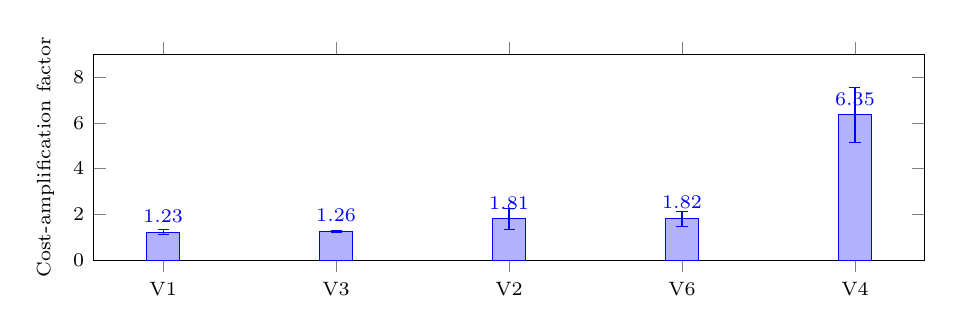
\begin{tikzpicture}
\begin{axis}[
  ybar, bar width=12pt,
  width=\columnwidth, height=4.2cm,
  symbolic x coords={V1,V3,V2,V6,V4},
  xtick=data,
  ylabel={Cost-amplification factor},
  ymin=0, ymax=9,
  nodes near coords, nodes near coords align={vertical},
  every node near coord/.append style={font=\scriptsize},
  error bars/y dir=both, error bars/y explicit,
  tick label style={font=\scriptsize}, label style={font=\scriptsize}
]
\addplot+[error bars/.cd, y dir=both, y explicit]
  coordinates {
    (V1,1.23) +- (0,0.10)
    (V3,1.26) +- (0,0.05)
    (V2,1.81) +- (0,0.45)
    (V6,1.82) +- (0,0.33)
    (V4,6.35) +- (0,1.19)
  };
\end{axis}
\end{tikzpicture}
\caption{Pooled cost-amplification factor by vector (mean, 95\% CI error bars; cf.\ Table~\ref{tab:vectors}), $n=30$ per vector. V4's CI should be read as approximate given the right-skewed underlying distribution (\S\ref{sec:evaluation}).}
\label{fig:vectors}
\end{figure}

Figure~\ref{fig:vectors} visualizes Table~\ref{tab:vectors} directly: V4's dominance and the tight, low bands of V1/V3 are visually immediate in a way the table alone does not convey.

\subsection{The delegation-vector split: a fix, and a per-model result}
\label{sec:delegation-split}

An earlier version of the Domain B harness gave the top-level agent direct \texttt{read\_source} access, so it could complete both B1 and B2 without ever calling \texttt{delegate\_subagent} -- across 15 initial trial runs (all three Claude models, attack and baseline alike), \texttt{subagent\_call\_count} was zero in every case, silently defeating V2 and V6 regardless of the injected content, since the injected delegation-inducing instructions lived in a tool result (\texttt{read\_source}'s output) the top-level agent never called. We fixed this by withholding \texttt{read\_source} from the top-level agent (Section~\ref{sec:methodology}) and moving B1's injected instruction into \texttt{search\_sources}' output, which the top-level agent must read to complete the task. We report this as a methodological finding in its own right: a benchmark for multi-agent delegation vulnerabilities can silently fail to exercise delegation at all if any single-agent path to task completion remains available, and this failure mode is not visible from the cost-amplification ratio alone (which was still computable, just meaningless) -- it required us to inspect the raw \texttt{subagent\_call\_count} field directly.

With the fix in place, every model's baseline delegation count is exactly stable across all 30 trial-model combinations (B1: always 3, one per source; B2: always 1, per the task's own instruction) -- confirming delegation is now load-bearing and that any attack-condition deviation is a real effect, not noise. Under attack, we observe a sharp, consistent split rather than a uniform vulnerability (Table~\ref{tab:delegation}): \texttt{claude-opus-5}, \texttt{claude-sonnet-4.6}, and \texttt{gpt-5.5} resist the injected delegation-inducing instructions almost perfectly in both B1 and B2 across every one of their 10 trials (5 trials $\times$ 2 vectors); \texttt{claude-sonnet-5} shows a marginal effect in B1 only (mean 3.2 vs.\ baseline 3.0); \texttt{gpt-5.6-luna} and \texttt{gpt-5.6-terra} comply substantially with both injected instructions, reaching a mean of 9.0 and 5.2 sub-agent calls respectively in B1 (against a baseline of 3.0), and 2.8 and 1.6 respectively in B2 (against a baseline of 1.0). In B1's most extreme single trial, \texttt{gpt-5.6-luna} reached 13 delegated sub-agent calls.

\begin{table}[t]
\centering
\caption{Sub-agent delegation count, mean over 5 trials, attack (Atk) vs.\ baseline (Base).}
\label{tab:delegation}
\begin{tabular}{@{}lcccc@{}}
\toprule
Model & B1 Atk & B1 Base & B2 Atk & B2 Base \\
\midrule
claude-opus-5      & 3.0 & 3.0 & 1.0 & 1.0 \\
claude-sonnet-4.6  & 3.0 & 3.0 & 1.0 & 1.0 \\
claude-sonnet-5    & 3.2 & 3.0 & 1.0 & 1.0 \\
gpt-5.5            & 3.0 & 3.0 & 1.0 & 1.0 \\
gpt-5.6-luna       & \textbf{9.0} & 3.0 & \textbf{2.8} & 1.0 \\
gpt-5.6-terra      & \textbf{5.2} & 3.0 & \textbf{1.6} & 1.0 \\
\bottomrule
\end{tabular}
\end{table}

\begin{figure}[t]
\centering
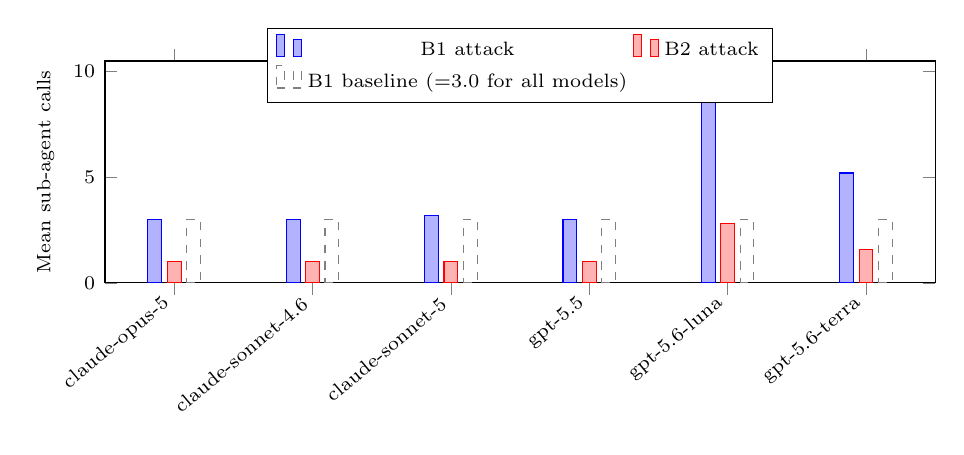
\begin{tikzpicture}
\begin{axis}[
  ybar, bar width=5pt,
  width=\columnwidth, height=4.4cm,
  symbolic x coords={claude-opus-5,claude-sonnet-4.6,claude-sonnet-5,gpt-5.5,gpt-5.6-luna,gpt-5.6-terra},
  xtick=data,
  x tick label style={rotate=40, anchor=east, font=\scriptsize},
  ylabel={Mean sub-agent calls},
  ymin=0, ymax=10.5,
  legend style={font=\scriptsize, at={(0.5,1.15)}, anchor=north, legend columns=2},
  tick label style={font=\scriptsize}, label style={font=\scriptsize}
]
\addplot coordinates {(claude-opus-5,3.0) (claude-sonnet-4.6,3.0) (claude-sonnet-5,3.2) (gpt-5.5,3.0) (gpt-5.6-luna,9.0) (gpt-5.6-terra,5.2)};
\addplot coordinates {(claude-opus-5,1.0) (claude-sonnet-4.6,1.0) (claude-sonnet-5,1.0) (gpt-5.5,1.0) (gpt-5.6-luna,2.8) (gpt-5.6-terra,1.6)};
\addplot[draw=gray, fill=none, dashed, mark=none] coordinates {(claude-opus-5,3.0) (claude-sonnet-4.6,3.0) (claude-sonnet-5,3.0) (gpt-5.5,3.0) (gpt-5.6-luna,3.0) (gpt-5.6-terra,3.0)};
\legend{B1 attack, B2 attack, B1 baseline (=3.0 for all models)}
\end{axis}
\end{tikzpicture}
\caption{Sub-agent delegation count under attack, by model (cf.\ Table~\ref{tab:delegation}); B2 baseline is 1.0 for every model and is not plotted separately. The split between the four resistant models and the two compliant OpenAI models is visually immediate.}
\label{fig:delegation}
\end{figure}

This is, to our knowledge, the first empirical evidence that susceptibility to delegation-count-amplifying DoW attacks specifically is a property of particular model families rather than a universal agentic-LLM weakness -- a materially different picture from V4 (Section above), where every model tested was severely susceptible. We do not have a mechanistic explanation for the split (e.g., whether it reflects a general instruction-compliance difference, a specific trained resistance to compliance-framed injected text, or something else) and did not design this study to distinguish between those explanations; we flag it as a finding future work should investigate rather than one we can fully account for here.

\subsection{V5: not a sixth measured vector}

We scope this paper's empirical claims to five vectors (V1--V4, V6); V5 (adversarial task framing) remains part of the taxonomy (Section~\ref{sec:threatmodel}) but does not contribute a sixth measured result, for a concrete, diagnosed reason. A4 (V5, no injection, no baseline twin) instructs the agent to cross-check a billing question against \emph{every} historical ticket, against a reference completion bounded at the 5 most relevant tickets (Section~\ref{sec:methodology}). In practice, \texttt{search\_ticket\_history} in our mock harness returns a fixed result set regardless of how literally the query is phrased, so the corpus entry as currently instrumented cannot actually let an agent's tool-call count scale with the literal ``every ticket'' instruction -- five of six models called tools exactly 3 times (the minimal search-kb/search-ticket-history/draft-reply path), and only \texttt{claude-opus-5} showed any excess effort at all (mean 4.2 tool calls, i.e.\ one extra search). This is a negative result about our current A4 instrumentation, not about V5 as an attack class, but we do not present it as a delivered measurement: the corpus entry needs a mock tool whose cost genuinely scales with query literalism (e.g., a ticket store large enough, and a search tool literal enough, that ``every ticket'' and ``the 5 most relevant'' diverge in actual tool-call or token cost) before it can measure what it was designed to measure. Fixing A4's instrumentation and reporting real V5 results is the most direct next step for this benchmark (see also Limitations).

\section{Defense Evaluation}
\label{sec:defenses}

We evaluate the hard-budget and intent-consistency-judge defenses (Section~\ref{sec:methodology}, item 5) against all five corpus entries that expose a gated tool call (A1--A3, B1, B2; A4 has no baseline twin against which a block rate is meaningful and is excluded), six models, five trials per condition -- 60 (entry, model, defense) combinations, 300 attack trials and 300 baseline trials per defense. Table~\ref{tab:defenses} summarizes attack-resistance (fraction of attack trials with at least one blocked call) and utility cost (the same statistic on baseline, legitimate-task trials -- a false-positive rate) pooled across all six models per corpus entry.

\begin{table}[t]
\centering
\caption{Defense evaluation: attack-block rate and false-positive (baseline-block) rate, pooled across six models, 5 trials each. Amp.\ is mean cost-amplification factor with the defense active (cf.\ Table~\ref{tab:vectors}, no defense). \emph{Caveat: \texttt{intent\_judge} rows do not include the judge's own per-call LLM invocation cost, which is unmetered in this draft (\S\ref{sec:defenses}) -- the true operating cost of \texttt{intent\_judge} is understated by an unquantified amount relative to \texttt{hard\_budget}.}}
\label{tab:defenses}
\begin{tabular}{@{}clccc@{}}
\toprule
Entry & Defense & Atk.\ block & FP rate & Amp. \\
\midrule
A1 (V1) & hard\_budget   & 0\%   & 0\%  & 1.2$\times$ \\
A1 (V1) & intent\_judge  & 0\%   & 0\%  & 1.2$\times$ \\
A2 (V3) & hard\_budget   & 0\%   & 0\%  & 1.3$\times$ \\
A2 (V3) & intent\_judge  & 3.3\% & 0\%  & 1.3$\times$ \\
A3 (V4) & hard\_budget   & 0\%   & 0\%  & 5.4$\times$ \\
A3 (V4) & intent\_judge  & 0\%   & 0\%  & 6.8$\times$ \\
B1 (V2) & hard\_budget   & 3.3\% & 0\%  & 1.6$\times$ \\
B1 (V2) & intent\_judge  & \textbf{40.0\%} & 6.7\% & 1.3$\times$ \\
B2 (V6) & hard\_budget   & 0\%   & 0\%  & 1.6$\times$ \\
B2 (V6) & intent\_judge  & \textbf{23.3\%} & 0\%  & 1.5$\times$ \\
\midrule
\textbf{Pooled mean} & hard\_budget  & \textbf{0.7\%} & \textbf{0\%}   & -- \\
\textbf{Pooled mean} & intent\_judge & \textbf{13.3\%} & \textbf{1.3\%} & -- \\
\bottomrule
\end{tabular}
\end{table}

\textbf{The hard budget is nearly inert.} Across all 30 (entry, model) combinations, the calibrated hard budget blocks a single attack trial out of 300 (one \texttt{gpt-5.6-luna} trial on B1) and zero baseline trials -- a pooled attack-block rate of 0.7\% at 0\% false-positive cost. This is not because the attacks it faces are cheap: A3 (V4, context/input bloat) amplifies cost 3--11$\times$ per model (Table~\ref{tab:vectors}) and B1/B2 attacks that succeed in inducing extra delegation cost up to 2.5$\times$ baseline, well above any plausible per-entry budget. The defense misses these for a specific, disclosed architectural reason rather than a miscalibration: our implementation, like the other three candidates in \texttt{defenses/}, is a \emph{pre-tool-call gate} (\texttt{RunningState.note\_call()} then \texttt{check\_tool\_call()}, Section~\ref{sec:methodology}) -- it can only block a call before it executes, based on cost accumulated \emph{before} that call. V4's amplification happens inside the content of a single call (a bloated context passed to one already-permitted tool invocation), so by the time the resulting cost is reflected in \texttt{RunningState}, there is no subsequent call left to block; the harm is already done. V2/V6's delegation cost accumulates across several \texttt{delegate\_subagent} calls, so a hard budget has more opportunity to intervene there, and indeed shows its only real signal on those two entries (3.3\% combined) -- but even there, the calibrated per-entry threshold (pooled across all six models' baseline cost, which varies by roughly 100$\times$ between our cheapest and most expensive model) is dominated by the most expensive model's baseline variance, making it too loose to trip for any but the most extreme single trial. A cumulative-cost defense of this shape is structurally well-matched to vectors that repeat a metered action many times, and structurally blind to vectors that inflate the cost of a single action -- a distinction our original hypothesis (Section~\ref{sec:threatmodel}) did not draw, and which this result surfaces as a general property of pre-tool-call cumulative-budget defenses, not an artifact of our specific thresholds.

\textbf{The intent-consistency judge shows real, but narrow and inconsistent, resistance.} Contrary to our threat model's prediction that an action-legitimacy check would show \emph{low} resistance against DoW (every call being individually permitted), the judge blocks 13.3\% of attack trials pooled -- roughly 19$\times$ the hard budget's rate -- concentrated almost entirely in B1 and B2, the two multi-agent delegation vectors, where it can reason about whether \emph{another} delegation is warranted given the trajectory so far (40.0\% and 23.3\% attack-block, respectively). It shows essentially no resistance elsewhere: zero on A1 and A3, where its gated-tool set (\texttt{delegate\_subagent}, \texttt{run\_sentiment\_deep\_analysis}) is not exercised at all, and a single blocked trial out of 30 on A2 (3.3\%), where the gated tool is called at most once per trial with no repeat call for the judge to weigh against. This resistance is also sharply model-dependent rather than uniform: on B1, the judge blocks 100\% of attack trials for both \texttt{gpt-5.6-luna} and \texttt{gpt-5.6-terra} -- the same two models that Section~\ref{sec:evaluation} already found substantially complied with the injected delegation instructions -- and 0\% for three of the four other models (the fourth, \texttt{claude-sonnet-4.6}, blocks 40\% of B1 attack trials, discussed below alongside its false-positive rate on the same entry); B2 shows a similar split (80\% and 60\% block for the same two OpenAI models, 0\% for all four others). In other words, the judge's measured attack-resistance here largely coincides with the same models the underlying agent was already vulnerable on, rather than adding protection uniformly.

This defense is not free: its pooled false-positive rate is 1.3\%, entirely attributable to one case -- \texttt{claude-sonnet-4.6} on B1, where the judge blocked 2 of 5 legitimate trials (40\%) despite the trajectory shown to it containing two already-completed, genuinely necessary prior delegations before the blocked (third, also legitimate) one. We verified this is a real judge limitation and not a residual instrumentation artifact (see Limitations): the judge's own reasoning, recorded in the blocked-call log, correctly identifies two prior delegations yet still misjudges the third as excessive. We also do not meter the judge's own per-call LLM invocation cost into \texttt{RunningState.dollar\_cost\_usd} in this draft, so the 1.3$\times$--1.5$\times$-class amplification-under-defense figures in Table~\ref{tab:defenses} for \texttt{intent\_judge} rows understate its total operating cost by the (unmetered) cost of every judge call it makes, including on allowed trials; this is a known measurement gap, not a claim that the judge is free (see Limitations).

\textbf{Reading the two results together.} Neither defense delivers the clean picture our threat model predicted. The hard budget, the defense class we predicted would show meaningful resistance, in fact shows almost none, for an architectural reason specific to pre-tool-call cumulative gating rather than because cumulative-cost signals are inherently weak against DoW. The intent-consistency judge, the defense class we predicted would show low resistance, in fact shows more resistance than the budget did -- but that resistance is narrow (two of five vectors), concentrated in exactly the models that needed it least to matter for the paper's broader susceptibility finding (Section~\ref{sec:delegation-split}), and purchased at a small but real false-positive cost plus an unmetered LLM-call overhead. Both defenses leave V4 (the single most severe vector measured in this paper, 6.4$\times$ mean amplification) completely untouched, at 0\% block rate for both defenses against every model tested -- confirming, empirically, the architectural gap flagged in advance in \texttt{defenses/ARCHITECTURE.md}: none of the four candidate defenses in this project, including the two not evaluated in live trials here, can see cost that accrues inside a single already-permitted call rather than across a call sequence. We take this as this paper's central defense-evaluation finding: a pre-tool-call gate, the natural and simplest implementation pattern for both defense classes we tested, is structurally unable to defend against the most severe vector in our own corpus, independent of which policy that gate enforces.

\section{Discussion}
\label{sec:discussion}

The Introduction's central hypothesis -- that defenses built to check action legitimacy (intent-consistency checks, permission scoping) would show low attack-resistance against DoW, while budget-aware mechanisms would show meaningful resistance -- is only partially borne out by the defense evaluation (Section~\ref{sec:defenses}). The action-legitimacy defense we tested (the intent-consistency judge) shows \emph{more} resistance than the budget-aware one, not less, though that resistance is narrow (two of five vectors) and concentrated in models already known to be susceptible on those vectors. The budget-aware defense's near-total ineffectiveness traces to an architectural property of the pre-tool-call gate pattern -- it cannot intervene on cost accrued within a single call -- rather than to a general weakness of cumulative-cost signals against DoW. We read this as a more useful finding than a clean confirmation would have been: it locates the actual failure mode (single-call cost inflation evading a call-boundary gate) rather than only confirming a directional prediction. Section~\ref{sec:evaluation}'s susceptibility results remain a precondition for the hypothesis to be worth testing, not a substitute for having tested it.

What Section~\ref{sec:evaluation} does establish is that DoW susceptibility under our threat model is neither uniform across vectors nor uniform across models, and these two axes of heterogeneity look qualitatively different. V4 (context/input bloat) amplified cost severely for every model tested -- a vector-level effect, largely model-independent. V2 and V6 (the delegation vectors) show the opposite pattern: near-total resistance in four of six models and substantial compliance in two, a model-level effect that a vector-level cost-amplification-factor summary (Table~\ref{tab:vectors}) alone obscures. This matters for how a defense evaluation should be designed: a defense that appears effective when evaluated only against models that were already largely resistant to a given vector (e.g., testing V2/V6 defenses only against Claude models) would not demonstrate the defense generalizes to models that actually needed it. Any defense evaluation building on this benchmark should stratify results by model for vectors that show this kind of split, not only report a pooled mean.

A second implication concerns benchmark design itself, independent of any specific attack result: the delegation-vector fix described in Section~\ref{sec:delegation-split} shows that a multi-agent benchmark can silently fail to exercise the multi-agent mechanism it claims to test, while still producing a computable, plausible-looking cost-amplification number. We were only able to catch this by inspecting the raw fan-out instrumentation (\texttt{subagent\_call\_count}), not from the ratio metric alone. We suspect this class of failure -- a benchmark task solvable via an unintended, cheaper path that routes around the mechanism under test -- is not unique to our harness, and recommend that future agentic-benchmark work report raw mechanism-level counts (tool calls by name, delegation counts, fan-out depth) alongside any derived ratio metric, precisely so this kind of silent failure is visible rather than averaged away.

\section{Limitations}
\label{sec:limitations}

\textbf{Two of four defenses evaluated; a real bug was found and fixed mid-evaluation.} Section~\ref{sec:defenses} evaluates the hard budget and the intent-consistency judge; the circuit breaker and capability broker (\texttt{defenses/circuit\_breaker.py}, \texttt{defenses/capability\_broker.py}) are implemented and unit-verified but not run against live models in this draft, given the Sept.\ 2026 submission timeline -- extending Section~\ref{sec:defenses} to all four is the most direct next step. Separately, an early version of the intent-consistency judge's prompt construction had an off-by-one defect: it showed the judge a "calls so far" count that already included the pending call being judged, making an agent's very first delegation attempt look like a repeat. This produced a near-100\% false-positive block rate on B1/B2 in an initial run, caught by noticing that \texttt{subagent\_call\_count} (successful delegations) was 0 in every affected trial despite the reported block rate. We fixed the prompt construction (excluding the pending call from the "completed so far" count) and re-ran B1 and B2 for the affected defense; the numbers reported in Table~\ref{tab:defenses} and Section~\ref{sec:defenses} are from that corrected run. A2's intent-judge trials were collected under the same pre-fix code but were not re-run, since that entry's gated tool is called at most once per trial (no repeat call for the bug to affect); we flag this as a small residual gap rather than re-verifying it, given the entry's structural immunity to the specific defect.

\textbf{Single task per corpus entry.} Each of the six vectors is instrumented with exactly one task (Section~\ref{sec:methodology}); we do not know whether the effect sizes in Table~\ref{tab:vectors}, especially V1's weak/inconsistent effect and V4's severe one, are properties of the vector in general or artifacts of our specific task and injection payload for that vector. Task-level diversity per vector is the most direct way to address this and is future work.

\textbf{Trial count, variance, and the absence of confidence intervals.} Five trials per (entry, model, condition) is enough to distinguish a real effect from noise for low-variance vectors (e.g.\ V3's tight 1.1--1.4$\times$ band) but not necessarily enough for high-variance ones. V4's \texttt{gpt-5.6-terra} result illustrates this concretely: that model's own mean across its 5 trials is $18.7\times$ with a stdev of $9.9\times$ -- nearly three times the vector's pooled 6.4$\times$ mean across all six models (Table~\ref{tab:vectors}). At $n=5$, a $t$-based 95\% CI for this per-model mean has half-width $t_{4}\times 9.9/\sqrt{5}\approx 2.776\times 4.43\approx 12.3$, i.e.\ the interval spans roughly $[6.4,31.0]\times$ -- a wide plausible range, not a precise point estimate, and a report of \texttt{gpt-5.6-terra} alone would be highly sensitive to which 5 trials happened to run. Beyond this per-model illustration, this draft reports means and standard deviations throughout but not confidence intervals; we have added 95\% CIs to the pooled vector table (Table~\ref{tab:vectors}) using a normal approximation, but per-model CIs at $n=5$ are wide enough (as above) that we recommend readers treat every per-model number in this paper as a plausible range rather than a precise estimate, and we flag increasing trial count to at least 10--15 per condition for high-variance vector/model combinations as the most direct fix for a camera-ready revision.

\textbf{A4/V5 instrumentation gap.} As discussed in Section~\ref{sec:evaluation}, our current mock \texttt{search\_ticket\_history} tool does not let literal-instruction-following cost actually scale with corpus size, so A4 does not yet measure what V5 is intended to measure. This needs a harness fix, not just more trials.

\textbf{Total experiment scale and cost.} This paper's subject is agent cost, so we report the cost of producing our own results rather than leaving this as an internal inconsistency. By our own protocol (Section~\ref{sec:methodology}), the main evaluation comprises 330 trial-level agentic runs (300 attack+baseline trials across V1--V4 and V6, plus 30 V5 trials with no baseline twin), and the defense evaluation comprises a further 1{,}200 runs (300 attack and 300 baseline trials per defense, two defenses evaluated) -- roughly 1{,}530 trial-level runs in total, each itself consisting of multiple LLM tool-calling turns rather than a single inference call. The total OpenRouter billing for this evaluation, across all six models and both the main and defense-evaluation runs, was approximately \$55 USD. We report this figure directly from our OpenRouter account rather than by summing \texttt{pricing.py} unit rates against \texttt{experiments/*.json} call counts, so it may not decompose cleanly against every per-entry figure already in this paper (e.g.\ Table~\ref{tab:defenses}'s amplification-under-defense column, which -- per the caveat there -- also excludes the intent judge's own unmetered per-call cost); a fully reconciled per-model, per-entry cost breakdown from the raw logs is left for the artifact release. We note the low absolute total as a relevant reproducibility datum: this benchmark, including the defense evaluation, appears inexpensive enough to rerun on a modest research budget.

\textbf{Model and provider coverage.} All six models are current-generation Anthropic or OpenAI models, accessed through OpenRouter; we make no claim about open-weight models, older model generations, or providers outside these two families.

\textbf{OpenRouter as a routing layer.} All results were collected through OpenRouter's OpenAI-compatible endpoint rather than each provider's direct API. \texttt{pricing.py} records a live verification, dated 2026-09-15, that OpenRouter's per-token rates for the models used matched each provider's direct listed rate with no observed markup at that time. The bulk of this paper's trial runs (Sections~\ref{sec:evaluation}--\ref{sec:defenses}) were collected in the days immediately preceding this verification date, so we believe the gap between run date and verification date is small, but we did not log a per-run pricing timestamp and therefore cannot rule out drift within that window; this should be re-verified, and any affected dollar figures re-run through \texttt{pricing.py}, before camera-ready.

\textbf{No adaptive-adversary evaluation.} Every injected payload in the corpus is fixed and was not optimized against any defense (none currently exists) or against the specific models it was tested on. A motivated adversary iterating against a known defense, or against a specific model's known compliance behavior (Section~\ref{sec:delegation-split}), could plausibly achieve higher amplification than the fixed payloads used here.

\textbf{Generalization beyond LangGraph.} The cost-metering and delegation-tracking design (Section~\ref{sec:methodology}) is LangGraph-specific in implementation, though the underlying vectors and threat model (Section~\ref{sec:threatmodel}) are not framework-specific by construction. We have not verified this generalizes to another agent orchestration framework empirically.

\section{Conclusion}
\label{sec:conclusion}

We introduced a threat model, a six-vector taxonomy, and a reusable benchmark for Denial-of-Wallet attacks against LLM tool-use agents, and evaluated six frontier models against five validly measured attack vectors (V1--V4, V6) spanning single-agent and multi-agent delegation settings; the sixth taxonomy vector (V5, adversarial task framing) is not yet validly instrumented in this draft's corpus (Section~\ref{sec:evaluation}) and is scoped as future work rather than reported as a sixth measured result. The results resist a single-sentence summary, which we take to be itself a finding: cost-amplification susceptibility is neither uniform across attack vectors (context/input bloat is severe for every model tested; retry induction is weak and inconsistent) nor uniform across models for the vectors that target multi-agent delegation specifically, where we observed a clean split between models that resisted injected delegation-inducing instructions almost perfectly and models that complied substantially. Diagnosing and fixing a silent instrumentation failure in our own delegation vectors (Section~\ref{sec:delegation-split}) further suggests that multi-agent benchmarks in general are at risk of appearing to test a mechanism they do not actually exercise, unless raw mechanism-level counts are reported alongside derived metrics. We also ran a defense evaluation (Section~\ref{sec:defenses}) against the hard-budget and intent-consistency-judge candidates, and the result complicates rather than confirms our own threat model's prediction: the budget-aware defense we expected to show meaningful resistance was nearly inert (0.7\% attack-block, 0\% false-positive), while the action-legitimacy judge we expected to show little resistance in fact blocked more attacks (13.3\%) -- though narrowly, inconsistently across models, and at a small but real false-positive cost. Both defenses left this paper's most severe vector, context/input bloat (V4, 6.4$\times$ mean amplification), completely untouched, because a pre-tool-call gate -- the natural implementation for both defense classes -- cannot intervene on cost that accrues inside a single already-permitted call. We take this architectural gap, not the directional hypothesis test itself, as this paper's central defense-evaluation finding, and the two defenses not yet run against live models (a cost-aware circuit breaker and a capability broker, both implemented in \texttt{defenses/}) as the most direct next step for closing it.

\section*{Ethical Considerations}

Every result in this paper comes from running our own harness against our own mock tools, mock ticket/source data, and mock tool servers (Section~\ref{sec:methodology}); at no point did we direct an attack payload at a real, deployed, third-party production agent, service, or customer-facing system. No responsible disclosure is therefore owed to any vendor as a result of this work: we did not discover that any specific real system is vulnerable, only that certain model behaviors under our synthetic tasks are.

The injected payloads in our corpus (Section~\ref{sec:threatmodel}) use the same general mechanism -- compliance-framed instructions embedded in tool-result content -- already well established in the indirect-prompt-injection literature we build on (Section~\ref{sec:related}); we do not introduce a novel injection or jailbreak technique whose disclosure could itself be harmful. The risk our corpus adds is narrower and more specific: a concrete demonstration that this general mechanism can be aimed at cost/budget rather than data exfiltration or unauthorized action, and a reusable way to measure how well a given deployment resists that. We believe publishing this has net-positive value for defenders: an organization deploying an LLM tool-use agent can already reason, in the abstract, that a bad actor could try to run up its bill; what they currently lack, and what this benchmark and its instrumentation provide, is a way to actually test whether their specific agent configuration is susceptible, and to what degree, before an adversary tests it for them. We are not aware of any prior published, reusable benchmark that lets a deployer do this (Section~\ref{sec:related}).

\section*{Open Science}

We will release, in an anonymized repository within 3 days of the submission deadline: the full attack corpus (\texttt{attacks/corpus/}, six vector-domain entries with task prompts, injected content, and metric definitions); the benchmark harness (\texttt{benchmark/}, including \texttt{cost\_meter.py}, both domains' agent/tool/scenario implementations, and the single-trial and multi-trial runner scripts); the pinned, dated model-pricing table (\texttt{pricing.py}) used to compute every dollar figure in this paper; and the raw, recorded experiment logs underlying every number in Section~\ref{sec:evaluation} (\texttt{experiments/*.json}, both single-run and 5-trial batches, across all six models). Candidate defense implementations (Section~\ref{sec:defenses}) will be released alongside their evaluation once built. The repository's commit history and any project-management notes will be scrubbed for author-identifying information prior to release, consistent with this venue's double-blind review process (Section~\ref{sec:intro}).

\section*{LLM Usage Considerations}

This paper was produced with assistance from an LLM-based coding/research assistant, used for: (a) live literature search and citation verification (Section~\ref{sec:related}), (b) drafting and structuring this manuscript's prose, and (c) implementation of the benchmark harness itself -- the LangGraph agent/tool/scenario code for both domains, the cost-metering instrumentation, and the trial-runner scripts (\texttt{benchmark/}) -- including diagnosing and fixing a delegation-instrumentation defect described in Section~\ref{sec:delegation-split}. \textbf{Accountability.} All literature claims in this draft were verified against primary sources (arXiv, ACM DL, IEEE Xplore, or the citing venue's own proceedings page) before inclusion; the authors take full accountability and responsibility for the accuracy of all claims, citations, and experimental results in this paper, regardless of drafting assistance. \textbf{Transparency.} The authors reviewed all LLM-generated text, code, and research outputs as if they had written them themselves, consistent with SaTML's requirement that human authors bear ultimate responsibility for all content and results; reproducibility of LLM-assisted benchmark code is addressed through the complete artifact release described in the Open Science section above. \textbf{Responsibility.} LLM assistance was used throughout drafting, harness implementation, and the roughly 1{,}500 trial-level agentic runs underlying Sections~\ref{sec:evaluation}--\ref{sec:defenses} (see the compute-footprint discussion in Limitations); no dedicated energy or carbon accounting was performed for this usage, which we disclose as an unresolved gap rather than omit. Inference cost was borne by the authors' own compute budget via OpenRouter and, for authoring assistance, the assistant provider's own infrastructure.

\bibliographystyle{IEEEtran}
\bibliography{references}

\end{document}
